\documentclass[a4paper, 10pt]{article}

\newcommand{\Title}{UNITN -- Esami SML}
\newcommand{\docversion}{v1.0.0}

\usepackage{settings/main.preamble}

\title{Esami \emph{commentati} di\\Programmazione Funzionale}
\subtitle{\texttt{print "Hello World{\textbackslash}n";}}

% arara: pdflatex: { shell: yes, synctex: no }
% arara: pdflatex: { shell: yes, synctex: yes }
% arara: latexmk:  { clean: partial }
% arara: clean:    { extensions: [lol, synctex.gz] }
\begin{document}
\maketitle
\vfill
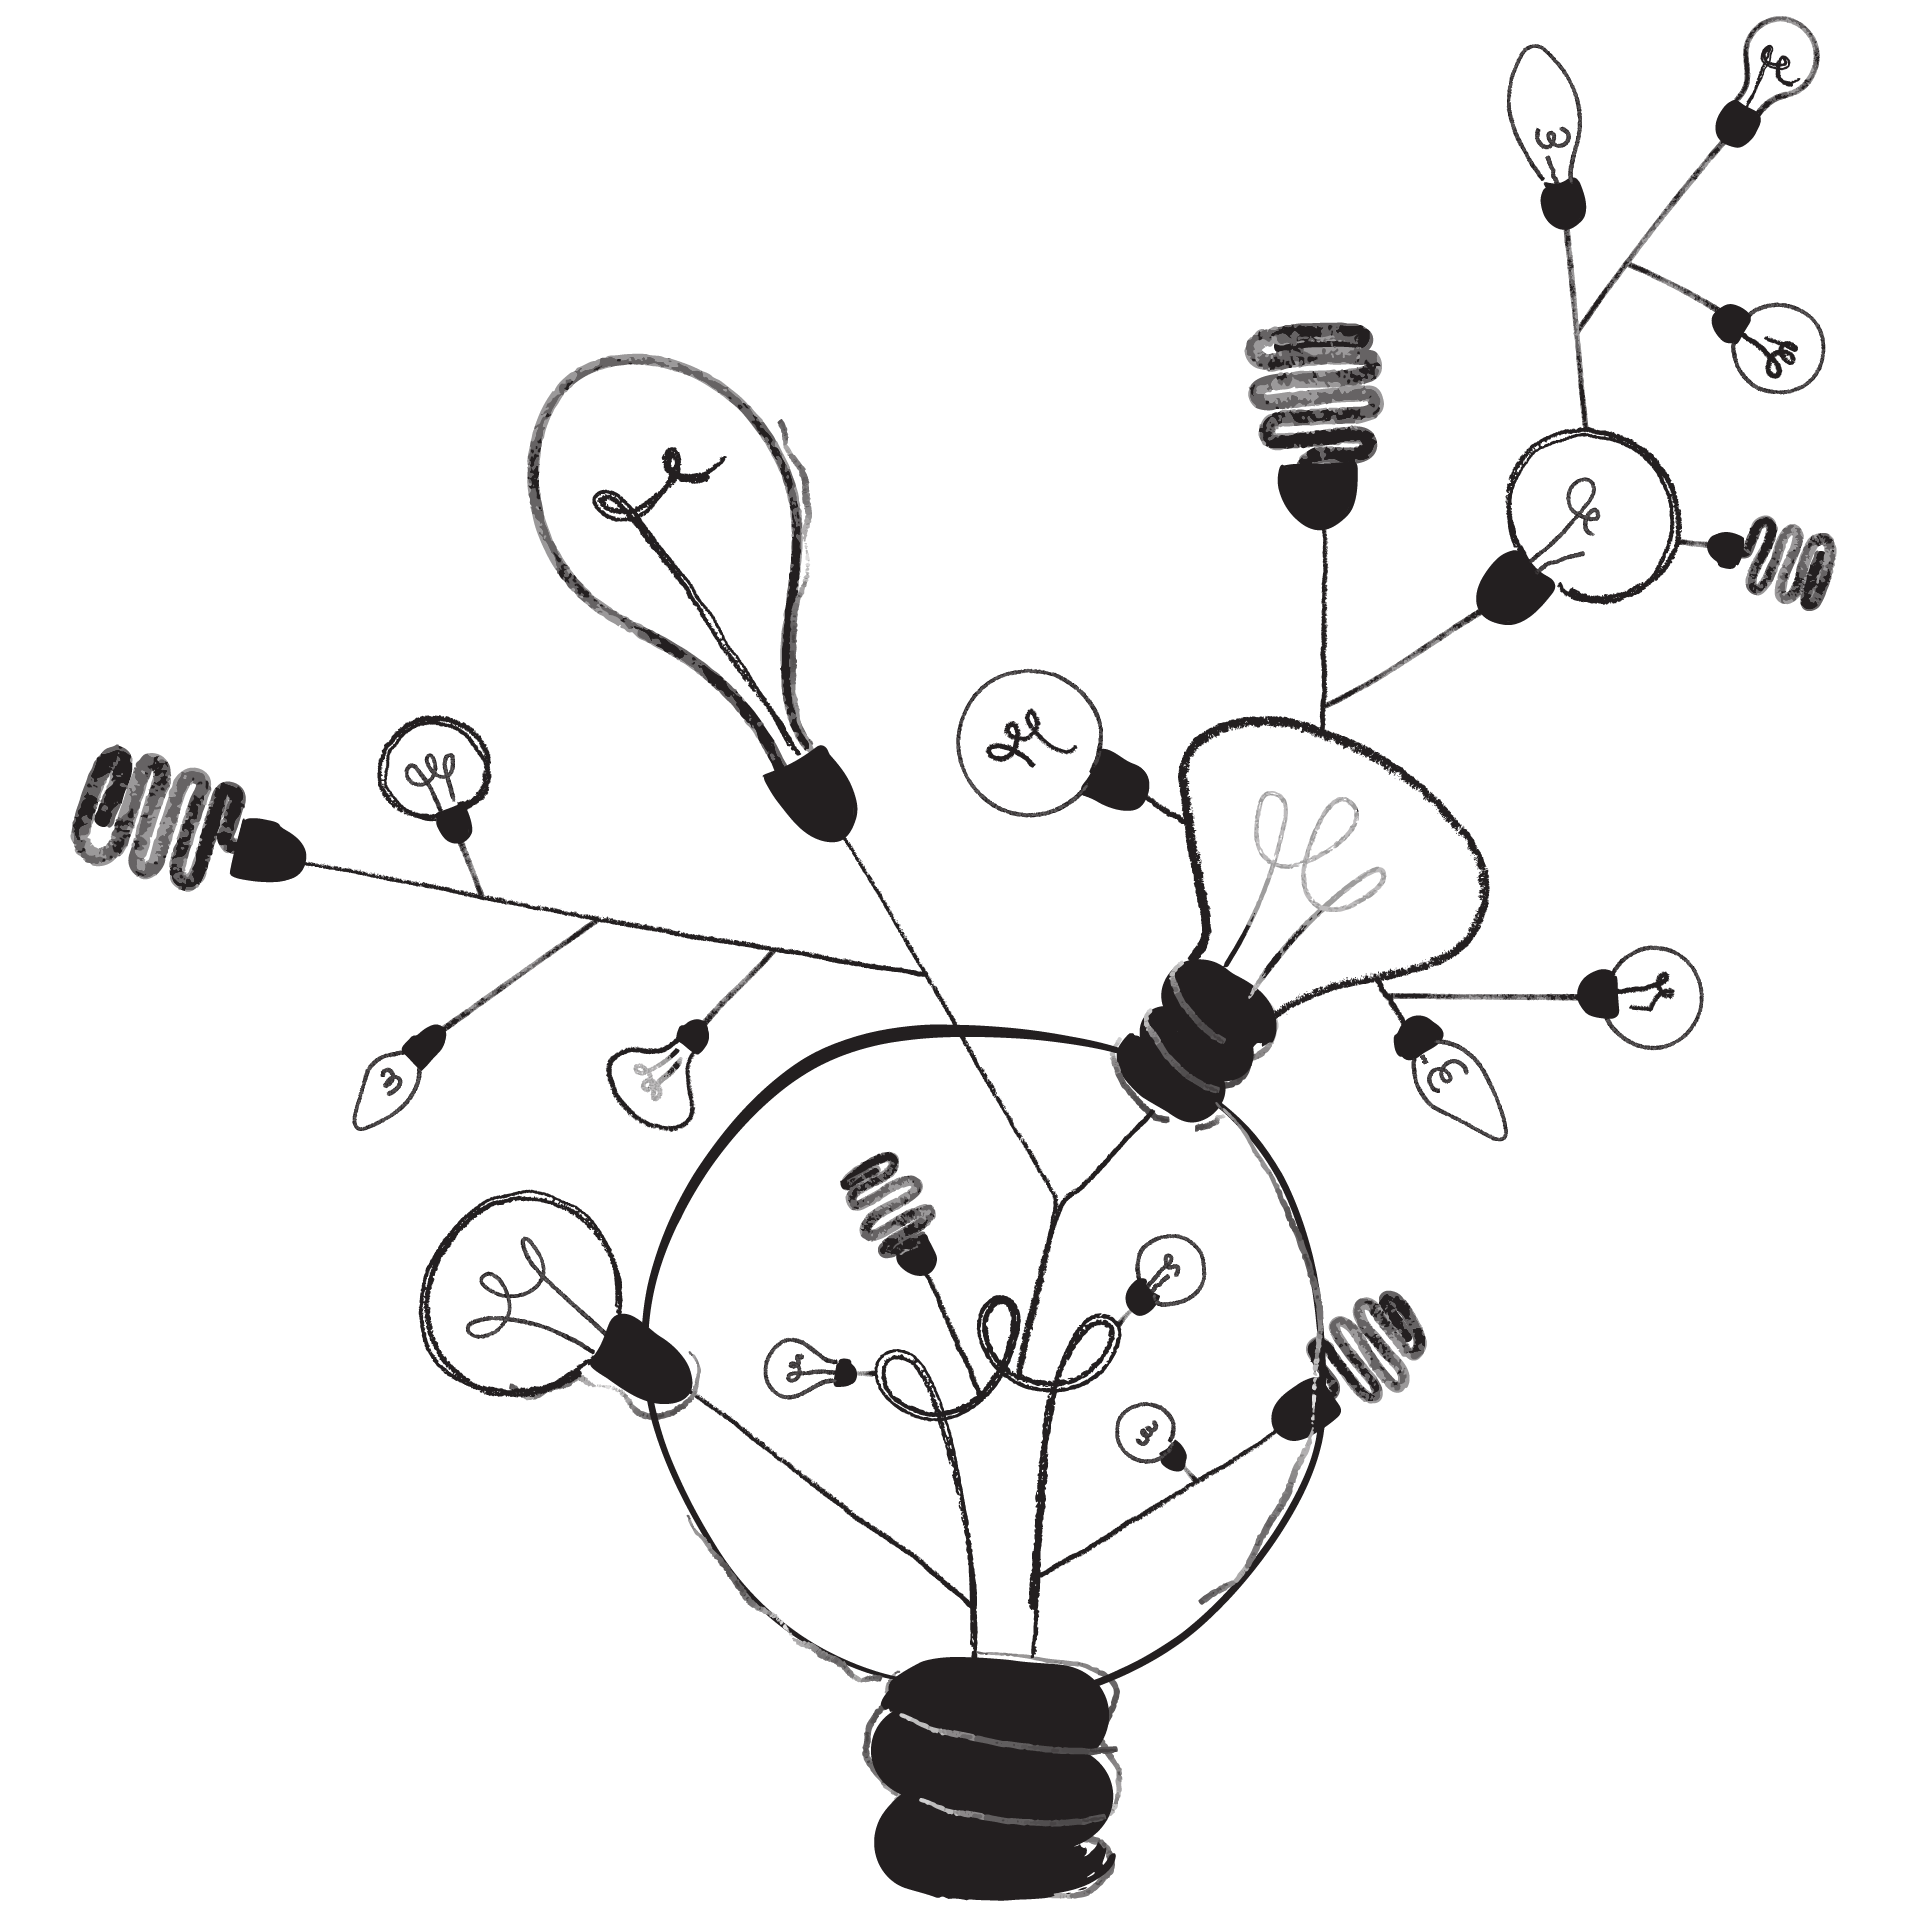
\includegraphics[width=.8\textwidth]{assets/figures/absurd-07}
\thispagestyle{empty}

\afterpage{\blankpage}
\clearpage

\pagestyle{pageReference}

\section*{Introduzione}

Lo scopo principale di questi appunti è quello di esaminare più da vicino gli esami di programmazione funzionale tenuti all'Università degli Studi di Trento. %
Questi appunti non sono completi, e la loro lettura non permette, da sola, di superare l’esame. %
La versione più recente si trova all'indirizzo:

\begin{center}
	\url{github.com/emanuelenardi/latex-sml}
\end{center}

% \subsection*{Donazioni}
%
% Questa dispensa è in fase di riscrittura, sudore e lacrime sono stati versati.
% Per supportare l'autore in questo lungo e tortuoso viaggio effettua una \href{https://paypal.me/pools/c/85MUW0ex8l}{piccola donazione{\ExternalLink}}.

% \subsection*{Ringraziamenti}
%
% Un grazie di cuore a:
% \begin{itemize}
% 	\item Riccardo Persico che dice -- ``Grazie''
% 	\item Alessio Gandelli che dice -- ``grazie per tutto''
% \end{itemize}

\subsection*{Materiale}

Puoi trovare una veloce introduzione a Standard ML su \href{https://learnxinyminutes.com/docs/standard-ml/}{Learn X in Y minutes \ExternalLink}.

\smallskip
Ho prodotto una \href{bit.ly/sml-youtube-playlist}{playlist di youtube{\ExternalLink}} che tratta gli argomenti del corso.
Se trovi qualche video esplicativo e pensi che possa tornare utile ai tuoi compagni di corso, tramite questo link, puoi aggingerli direttamente alla playlist.

\smallskip
Per tutto il resto consulta la cartella \href{https://bit.ly/drive-folder}{Google Drive{\ExternalLink}} del corso triennale di Informatica.

\subsection*{Segnalazione di errori}

Se hai trovato un errore ti prego di aprire un \href{github.com/emanuelenardi/latex-sml/issues/new}{\textsf{issue}{\ExternalLink}} su \faicon{github} github.

\section*{Riguardo l'autore}

\begin{minipage}[c]{.5\textwidth}
\centering
	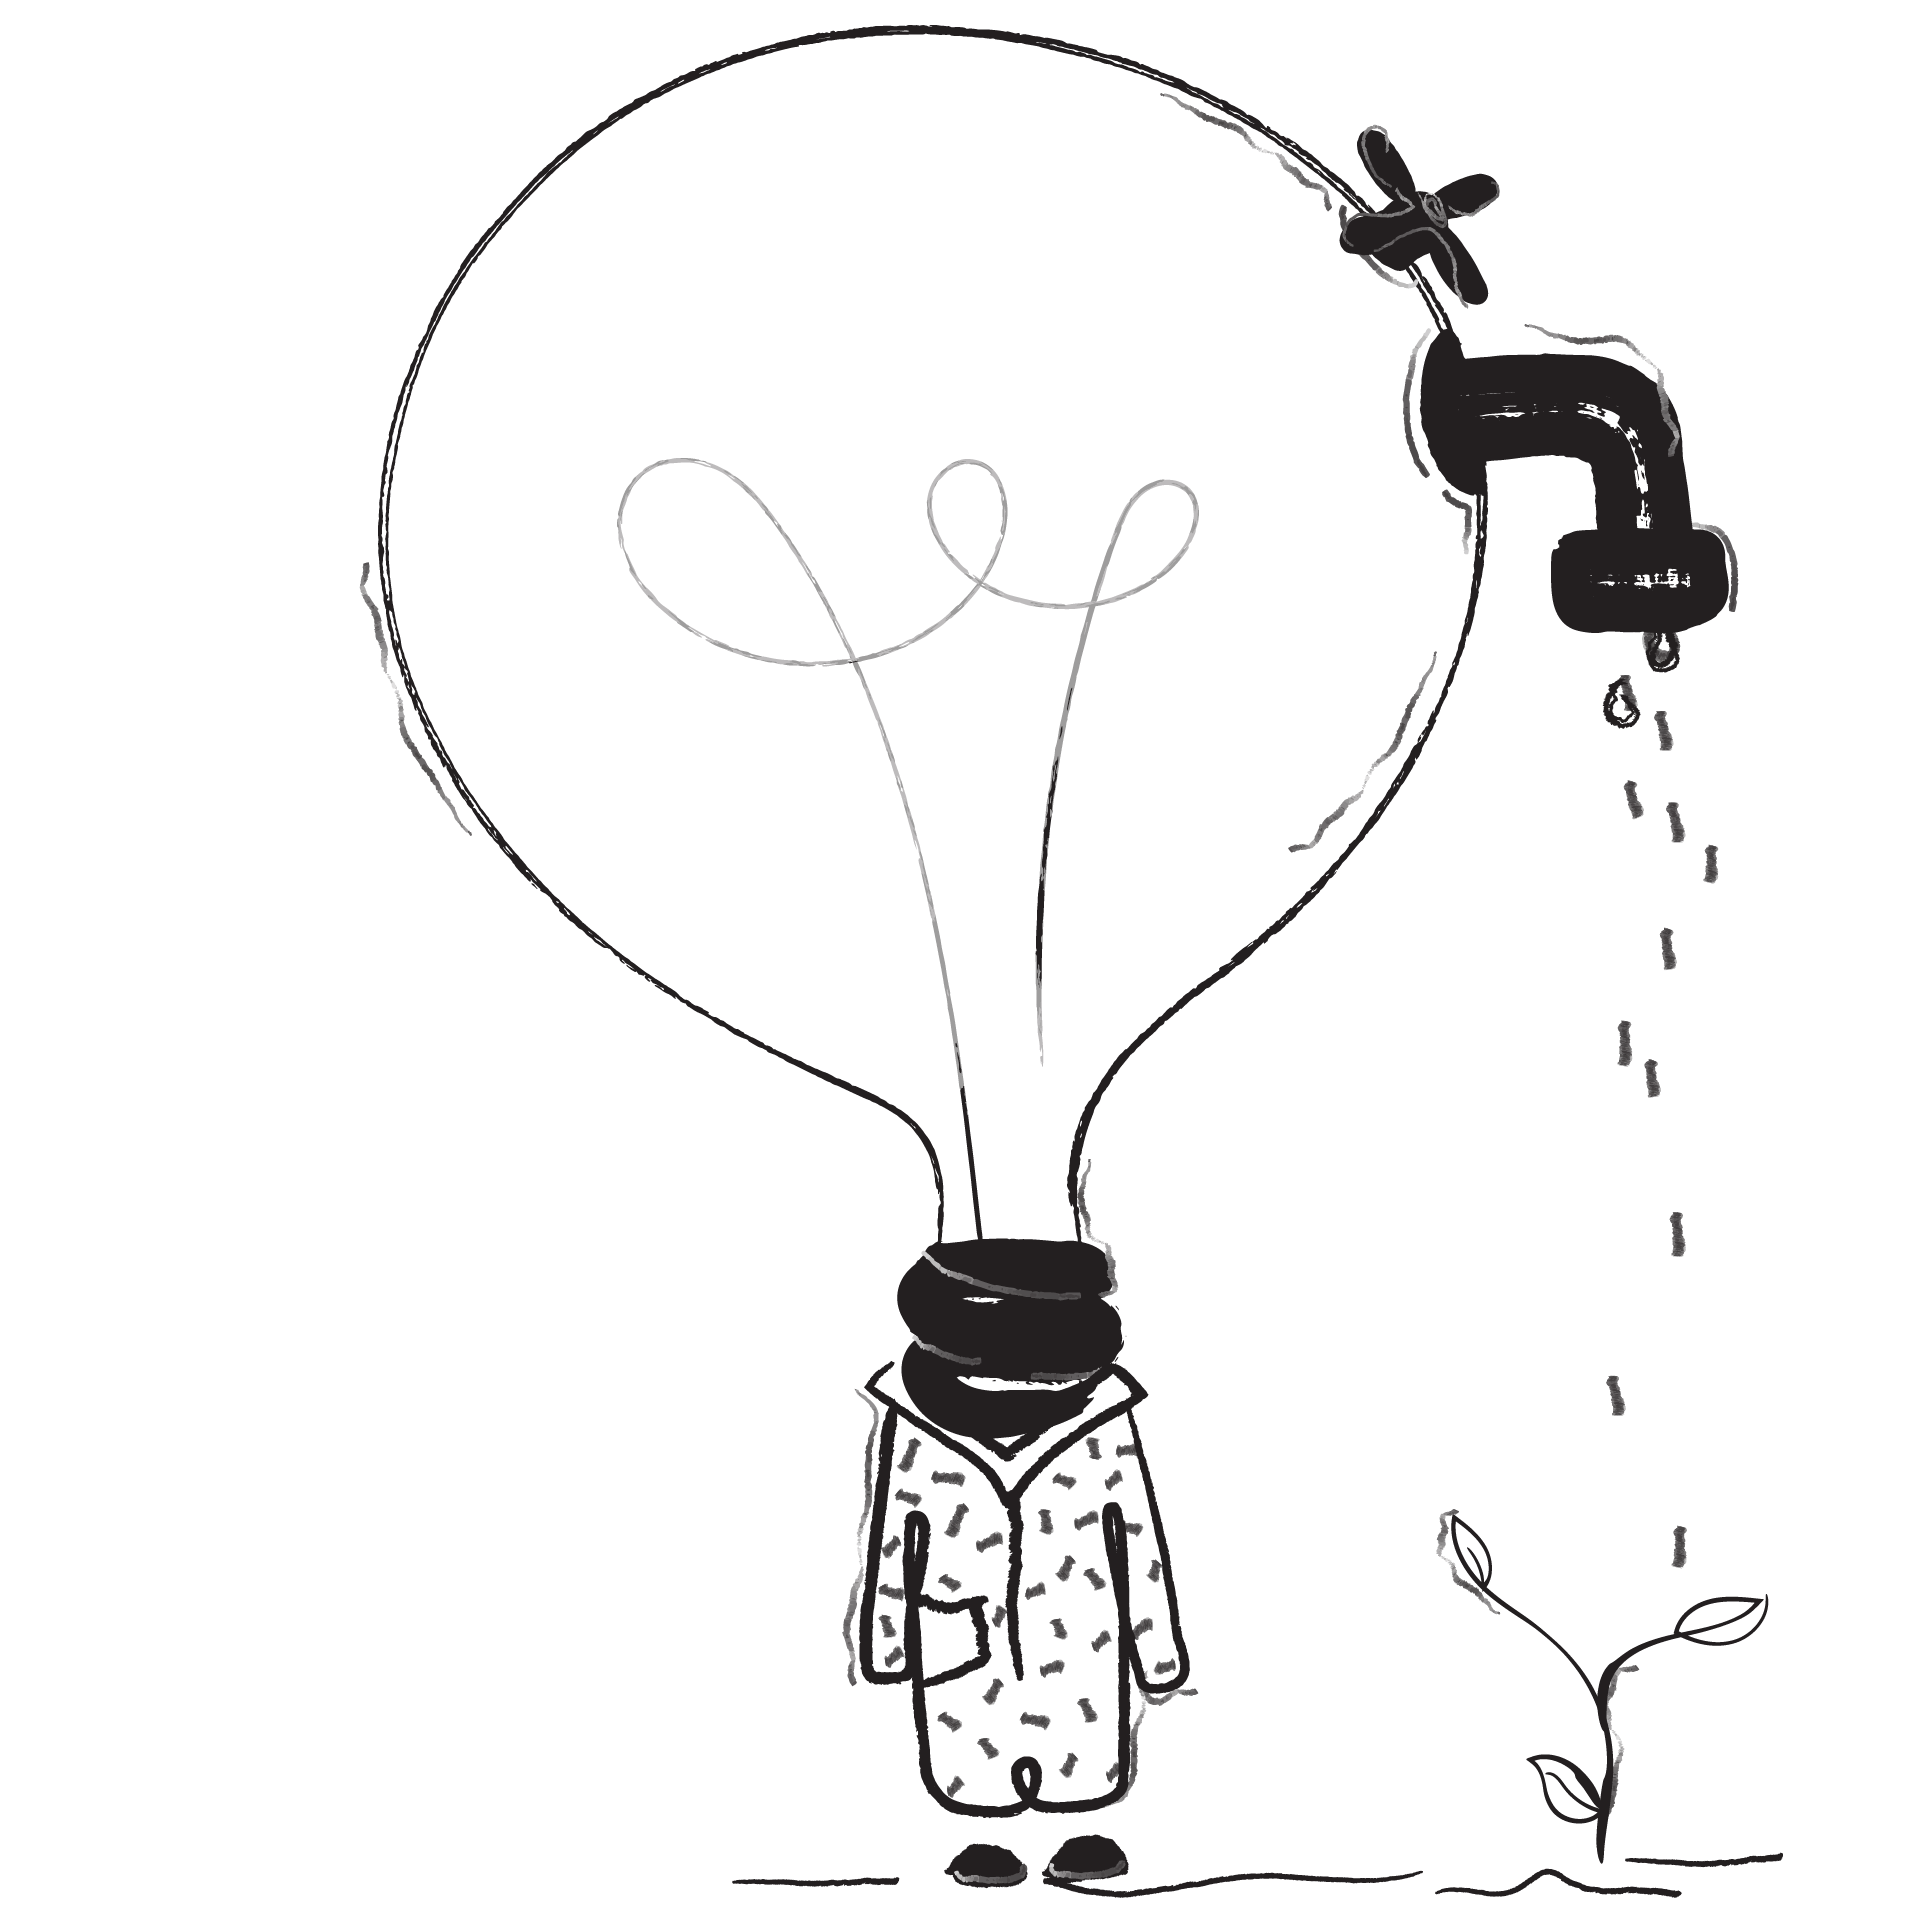
\includegraphics[width=0.8\textwidth]{assets/figures/absurd-08}
	\captionof*{figure}{---\em\ un autoritratto}
\end{minipage}
\begin{minipage}[c]{.5\textwidth}
	Emanuele Nardi è uno studente di informatica all'Università degli Studi di Trento, \href{https://www.facebook.com/rappresentantidisi/}{rappresentante degli studenti} e co-fondatore di \href{http://speckand.tech}{Speck\&Tech}.

	\medskip
	Appassionatosi al design alle superiori, nei primi anni di università scopre il programma di impaginazione {\LaTeX} con il quale inizia a prendere appunti durante le lezioni.
	Ha prodotto diverse dispense per il percorso di laurea triennale di informatica.

	\smallskip
	Tutti i suoi appunti sono disponibili sul suo \href{github.com/emanuelenardi}{profilo \faicon{github} github{\ExternalLink}}.
\end{minipage}


\afterpage{\blankpage}
\clearpage

\begin{multicols*}{2}
\microtypesetup{protrusion = false}
\fontsize{10pt}{12pt}\selectfont
\tableofcontents
\microtypesetup{protrusion = true}
\end{multicols*}

\begin{multicols*}{2}
\fontsize{10pt}{12pt}\selectfont
\listoflistings
\end{multicols*}

\section*{Come leggere questa dispensa}

\subsubsection{Letture consigliate}

Prima di prepararti alla prova pratica leggendo e provando questa dispensa ti consiglio di leggere ``\href{run:./intro-sml.pdf}{Introduzione a Standard ML}''.

\subsubsection*{Trial and Error}

Il Trial and Error è un modo comune e veramente efficace per imparare.
Al posto di chiedere aiuto su ogni piccola cosa, qualche volta spendere un po' di tempo da soli (a volte ore e giorni) e provare a far andare qualcosa ti aiuterà ad imparare più velocemente.

Se provi qualcosa e ti dà un errore, studia quell'errore.
Quindi prova a correggere il tuo codice.
Quindi prova a eseguirlo di nuovo. Se ricevi ancora un errore, modifica ancora il tuo codice.
Continua a provare e fallire finché il tuo codice non fallisce più.
Imparerai molto in questo modo leggendo questa dispensa, leggendo gli errori e imparando cosa funziona e cosa no. Provare, fallire, provare, fallire, provare, provare, provare, fallire, fallire, avere successo!

Questo è quanto hanno imparato molti ``pros''.
Ma non aver paura di chiedere aiuto, noi non mordiamo (duro).
L'apprendimento richiede tempo, i professionisti che hai incontrato non hanno imparato a diventare maestri in poche ore o giorni.

\subsubsection*{Indentazione}

L'indentazione è veramente importante! Il tuo codice funzionerà perfettamente senza, ma provocherà un grosso mal di testa a te e agli altri leggere il tuo codice.

Un breve spezzone di codice (25 linee o meno) probabilmente andrà bene senza indentazione, ma presto diventerà sciatto. \'E bene imparare ad indentare correttamente al più presto.
L'indentazione non ha uno stile definito, ma è meglio mantenere tutto coerente.

Per approfondimenti vedi la voce \href{https://en.wikipedia.org/wiki/Indentation_style}{``Indentation style''{\ExternalLink}} su Wikipedia.

\subsubsection*{Chiedere aiuto}

Prima di chiedere, prova a fare qualche ricerca tu stesso o prova a scrivere codice da solo.
Se ciò non ha prodotto risultati che ti soddisfano, leggi di seguito.

\begin{itemize}
	\item Non essere preoccupato di chiedere aiuto, anche le persone più intelligenti chiedono aiuto agli altri;
	\item Non essere preoccupato di mostrare quello che hai provato, anche se pensi che sia stupido (in particolare in questo caso, potresti aver trovato un modo più semplice di risolvere il problema);
	\item Posta qualsiasi cosa tu abbia provato;
	\item Fingi che chiunque tranne te sia un idiota e non sappia niente. Dai più informazioni possibili in modo da educare noi idioti su quello che stai cercando di fare;
	\item Aiutaci aiutati;
	\item Sii paziente, educato, aperto, gentile;
	\item Buon divertimento!
\end{itemize}

\renewenvironment{changelogitemize}
	{\begin{itemize}[label={}]}
	{\end{itemize}}

\begin{changelog}[
		% simple,
		sectioncmd=\section*,
		% title=Changelog,
		% label=sec:changelog,
		% author={}
]

\shortversion{v={Non rilasciato},
	changes={Aggiunto l'esame commentato di settembre 2015}
}

\shortversion{v=0.3.0, date=2019-05-09,
	changes={Aggiunto l'esame commentato di agosto 2015}
}

\shortversion{v=0.2.2, date=2019-05-05,
	changes={Aggiunto changelog}
}

\shortversion{v=0.2.1, date=2019-05-04,
	changes={Apportati cambiamenti all'introduzione}
}

\shortversion{v=0.2.0, date=2019-04-25,
	changes={Aggiunto l'esame commentato di giugno 2015}
}

\shortversion{v=0.1.0, date=2019-04-11,
	changes={Pubblicate nuove impaginazioni delle soluzioni d'esame}
}

\end{changelog}

\clearpage

\part{Esami Pratici}
\section{Giugno 2015}

\subsection{Testo}

Come noto, un numero naturale è esprimibile in base agli assiomi di Peano usando il seguente tipo di dato:
\lstinputlisting[
	style = SML,
	caption = {Definizione di numero naturale tramite gli Assiomi di Peano}
]{2015.06/nat.sml}

Usando tale tipo di dato, la \sml{somma} fra numeri naturali è esprimibile come:

\lstinputlisting[
	style = SML,
	caption = {Definizione della funzione \sml{somma} tramite gli Assiomi di Peano}
]{2015.06/nat_somma.sml}

Scrivere una funzione Standard ML, chiamata \sml{prodotto}, che ha tipo \sml{naturale -> naturale -> naturale}, che calcola il prodotto di due numeri naturali. Si noti che la funzione prodotto può usare la funzione somma nella sua implementazione.

\subsection{Guida alla soluzione}

Prendiamo confidenza con il tipo di dato definito:
\begin{lstlisting}[style = SML, caption = {Dichiarazione di numeri naturali}]
> zero;
val it = zero: naturale

> successivo(successivo zero);
val it = successivo (successivo zero): naturale
\end{lstlisting}

La \sml{somma} fra numeri naturali è esprimibile in due modi, equivalenti fra loro, un modo è quello illustrato dal professore, l'altro è il seguente:
\lstinputlisting[
	style = SML,
	caption = {Definizione \emph{alternativa} della funzione \sml{somma} tramite gli Assiomi di Peano}
]{2015.06/nat_somma_alt.sml}

\subsection{Commento sull'implementazione della funzione \sml{somma}}

Entrambe le definizioni di \sml{somma} sono corrette. Nella prima definizione il caso \emph{successivo a} restituisce una funzione che mappa una variabile \sml{n} nel successivo della somma di \sml{a} con \sml{n}, nella seconda definizione, invece, il caso \emph{successivo a} restituisce una funzione che mappa una variabile \sml{n} nella somma di \sml{a} con il successivo di \sml{n}.

\medskip
Il funzionamento dell'esecuzione della funzione \sml{somma} fra due numeri naturali -- definiti secondo gli Assiomi di Peano -- è la seguente:

\smallskip
bisogna togliere un valore \sml{successivo} al primo addendo affinché risulti pari al caso base (cioè zero). %
Questo lo si fa \textbf{o} aggiungendo un valore \sml{successivo} alla somma del primo addendo con il secondo (1\textsuperscript{a} implementazione) \textbf{o} sommando il primo addendo con il successivo del secondo addendo (2\textsuperscript{a} implementazione).
\begin{lstlisting}[style = SML, caption = {Esempio di esecuzione di \sml{somma}}]
> somma (successivo zero) (successivo (successivo zero));
val it = successivo (successivo (successivo zero)): naturale
\end{lstlisting}

La somma di 1 e 2, risulta 3.

\subsection{Soluzione}

N.B. sono state aggiunte delle parentesi per far sì che gli argomenti dati in pasto alla funzione \sml{somma} siano delle espressioni valutabili e non delle funzioni, quali sarebbero senza le parentesi.
\lstinputlisting[
	style = SML,
	caption = {Definizione della funzione \sml{prodotto} tramite gli Assiomi di Peano}
]{2015.06/nat_prodotto.sml}

\subsection{Esempio di esecuzione}

Mostriamo un esempio di esecuzione della funzione \sml{prodotto}:
\lstinputlisting[
	style = SML,
	caption = {Esempio di esecuzione}
]{2015.06/exec.sml}

\section{Luglio 2015}

\subsection{Testo d'esame}

Si consideri il seguente tipo di dato, che rappresenta una semplice espressione avente due argomenti \(x\) e \(y\):

\begin{listing}[!h]
\smlfile{assets/codes/2015.07/expr.sml}
\caption{Definizione di \texttt{Expr}}
\end{listing}

dove il costruttore \texttt{X} rappresenta il valore del primo argomento \texttt{x} dell'espressione,
il costruttore \texttt{Y} rappresenta il valore del secondo argomento \texttt{y},
il costruttore \texttt{Avg}, che si applica ad una coppia \texttt{(e1, e2)}, rappresenta la media (intera) dei valori di \texttt{e1} ed \texttt{e2},
mentre il costruttore \texttt{Mul} (che ancora si applica ad una coppia \texttt{(e1, e2)}) rappresenta il prodotto dei valori di due espressioni \texttt{e1} ed \texttt{e2}.

\medskip
Implementare una funzione Standard ML, chiamata \texttt{compute}, che ha tipo \texttt{Expr -> int -> int -> int}.

\medskip
Come suggerito dal nome, \texttt{compute} calcola il valore dell'espressione ricevuta come primo argomento, applicandola ai valori ricevuti come secondo e terzo argomento e ritorna un intero che indica il risultato finale della valutazione.

\medskip
\textbf{IMPORTANTE}: notare il tipo della funzione! Come si può intuire da tale tipo, la funzione riceve tre argomenti usando la tecnica del \emph{currying}. \'E importante che la funzione abbia il tipo corretto (indicato qui sopra). Una funzione avente tipo diverso da \texttt{Expr -> int -> int -> int} non sarà considerata corretta.

\subsection{Soluzione}

\begin{listing}[!h]
\smlfile{assets/codes/2015.07/compute.sml}
\caption{Definizione della funzione \texttt{compute}}
\end{listing}

\subsection{Guida alla soluzione}

Il problema si risolve con una funzione ricorsiva, che sfrutta la definizione del tipo di dato \texttt{Expr} e la tecnica  \emph{currying} per arrivare alla soluzione.
Nota come la definizione del tipo della funzione (\texttt{Expr -> int -> int -> int}) risulti un ottimo suggerimento per la risoluzione del problema.

La funzione individua 4 casi particolari: \texttt{X}, \texttt{Y}, \texttt{Avg(e1, e2)} ed infine \texttt{Mul(e1, e2)} tutti definiti in termini del dato \texttt{Expr}.
In ognuno dei casi vengono restituite due funzioni, le quali raccolgono i dati che verranno rielaborati nell'ultimo passaggio;
l'unico nella quale viene implementata la logica di calcolo.

\subsection*{Esempio di esecuzione}

Mostriamo un esempio di esecuzione della funzione \texttt{compute}:

\begin{listing}[!h]
\smlfile{assets/codes/2015.07/exec.sml}
\caption[]{Esempio di esecuzione}
\end{listing}


\begin{comment}
\newcommand*{\currentYear}{2019}

\foreach \year in {2015,2016,...,\currentYear}{%
	\foreach \month in {01,02,06,07,08,09}{%

		\IfFileExists{assets/exams/\year.\month} {%
			\input{assets/exams/\year.\month}%
			\newpage
		}{%
			% il file non esiste, quindi non fare nulla
		}%
	}%
}%
\end{comment}
\afterpage{\blankpage}
\clearpage

\section*{Conclusione}

Abbiamo raggiunto la fine del nostro viaggio, mio caro amico.
Spero che tu abbia imparato qualcosa.
Ma prima che te ne vada, considera di fare \href{https://paypal.me/pools/c/85MUW0ex8l}{una piccola donazione{\ExternalLink}}.

\medskip
Sei anche tu uno squattrinato studente fuori sede?
Ecco cosa puoi fare:
\begin{itemize}
	\item \emph{Correggere e segnalare} gli errori contenuti del testo e/o negli esercizi;
	\item Mettere una \faicon{star-o} sulla repository;
	\item Condividere questa dispensa con un compagno di corso.
\end{itemize}

% TODO testing
\hfill
\begin{minipage}[c]{.5\textwidth}
\centering
	
\includegraphics[width=0.8\textwidth]{assets/figures/absurd-06}
	% \captionof*{figure}{---\em\ un autoritratto}
\end{minipage}


\end{document}
